%======================================================================
% L04a_postulaty.pdf
%======================================================================
\section{Postuláty termodynamiky}
\strana{L04a-1}
\providecommand{\dbar}{\text{đ}}

\begin{itemize}
  \item dosavadní poznatky dovolují zformulovat základní postuláty TD tak, že termodyn.\ vlastnosti materiálu budou charakterizovány analytickými vlastnostmi entropie anebo vnitřní energie \\
  \textcolor{NavyBlue}{$\dd S = \frac1T\dd U - \sum_i\frac{y_i}{T}\dd X_i$; \ $[y_iX_i] = [U] = [T]$ \ \& \ $\Delta S|_{\text{izol}}\geq 0$}
\end{itemize}

lze nahlédnout z Clausiovy nerovnosti:
\[
  \oint\frac{\dbar Q}{T'}\leq 0 \ \Rightarrow\ \int_A^B\frac{\dbar Q}{T'} + \int_{B\,(\text{rev})}^A\frac{\dbar Q}{T}\leq 0 \quad\&\quad B\to A
\]
\[
  \Rightarrow\ \dbar Q\leq T\dd S \ \Rightarrow\ \vzorec{T\dd S\geq\dd U - \dbar W}
\]
$\to$ izol.\ systém $\Rightarrow$ $\dd U = 0$, $\dd X = 0$ $\Rightarrow$ $T\dd S\geq 0$
\[
  \Rightarrow\ \vzorec{[\dd S]_{U,\vec X}\geq 0 \quad\text{v nevratném procesu}}
\]
$\to$ systém v rovnováze tento stav již samovolně neopustí $\Rightarrow$ za daných externích podmínek již neexistuje spontánní nevratný proces

\begin{veta}[Podmínka rovnováhy izolovaného systému]
$(\Leftrightarrow)$ neexistují fluktuace \quad $[\delta S]_{U,\vec X_{\text{ext}}} > 0$

\medskip
\textbf{\sffamily\small i) For the equilibrium of any isolated system it is necessary and sufficient that in all possible variations of the state of the system which do not alter its energy, the variation of its entropy shall either vanish or be negative.} \hfill \textsc{Gibbs}
\end{veta}
%----------------------------------------------------------------------
\strana{L04a-2}
\begin{veta}[Postulát 1]
\textcolor{Red}{Existují rovnovážné stavy makroskopických systémů, které jsou plně charakterizovány hodnotou vnitřní energie $U$ a malým počtem dalších extenzivních proměnných.}
\end{veta}
\begin{itemize}
  \item[$\to$] v zásadě původní první a druhý axiom termodynamiky
  \item[$\to$] nerovnovážný stav je vždy specifikován větším počtem parametrů než rovnovážný (je třeba popsat nehomogenity, toky etc.), vždy ale méně než $6N$ -- kompletní specifikace mikrostavu
\end{itemize}

\begin{veta}[Postulát 2]
\textcolor{Red}{Existuje stavová funkce (entropie) extenzivních parametrů složeného systému, která je definována pro všechny rovnovážné stavy. Extenzivní parametry \underline{izolovaného} složeného systému bez vnitřních vazeb nabývají v rovnovážném stavu takové hodnoty, které odpovídají maximu entropie na prostoru všech rovnovážných stavů systému s libovolnými vnitřními vazbami. $S = S(U, X[1],\dots,X[k])$}
\end{veta}
\begin{itemize}
  \item[$\to$] krkolomný způsob, jak vyjádřit \uv{existuje funkce $S(U,X_1,\dots,X_n)$, která v rovnováze nabývá maxima}
  \item[$\to$] problém je, že mimo rovnováhu není $S$ definována, každý bod stavového prostoru je tedy třeba chápat jako rovnovážný stav, který se realizuje při nějakém vhodném nastavení vazeb/stěn ve složeném systému
  \item[$\to$] postulát vychází z poznatku, že $(\Delta S)_{\text{izol}}\geq 0$ \ \textcolor{NavyBlue}{$\Leftarrow \dbar Q\leq T\dd S$}
  \begin{itemize}
    \item[--] přechod do rovnováhy je svázán s nárůstem entropie, proces se zastaví až tehdy, když už není kam
  \end{itemize}
\end{itemize}

\noindent
\begin{minipage}{0.16\textwidth}\color{NavyBlue}\small Za chvíli přeformulujeme:\end{minipage}
\begin{minipage}{0.82\textwidth}
\begin{tcolorbox}[colback=NavyBlue!4,colframe=NavyBlue,boxrule=0.6pt,arc=1pt,left=4pt,right=4pt,top=2pt,bottom=2pt]
\color{NavyBlue}Rovnovážné hodnoty volných vnitřních extenzivních parametrů jsou takové, aby \underline{maximalizovaly entropii} pro danou hodnotu celkové vnitřní energie {\small (a ostatních vnějších ext.\ param.)}
\end{tcolorbox}
\end{minipage}

\begin{itemize}
  \item[$\to$] funkci $S = S(U,X_1,\dots,X_n)$ nazýváme \underline{(entropickou) \kw{fundamentální rovnicí}}
  \begin{enumerate}[label=\arabic*)]
    \item jednoznačně charakterizuje rovnovážný stav definovaný danými vazbami \textcolor{NavyBlue}{(hodnotami vnějších a vázaných vnitřních parametrů)}
    \item lze z ní odvodit $\forall$ relevantní stavové rovnice \quad \textcolor{NavyBlue}{$\dfrac{y_i}{T} = \Big(\pdv{S}{X_i}\Big)_{U,X_j}$}
  \end{enumerate}
\end{itemize}
\noindent\rule{\linewidth}{0.4pt}
%----------------------------------------------------------------------
\strana{L04a-3}
\begin{veta}[Postulát 3]
\textcolor{Red}{Entropie je spojitá diferencovatelná stavová funkce všech proměnných a je monotónně rostoucí funkcí $U$.}
\end{veta}
\begin{itemize}
  \item[$\to$] spojitost a diferencovatelnost implikuje, že $S$ má úplný diferenciál; tento postulát nám tedy říká, že v rovnovážném stavu si systém nepamatuje historii ($\int\dd S$ nezávisí na trajektorii)
  \item[$\to$] $\Big(\pdv{S}{U}\Big)_{X_i} > 0 \ \Leftrightarrow\ T > 0$ \\
  \dots\ existují systémy, kde to neplatí (omezený mikroskopický hamiltonián), ale TD s nimi neumí moc dobře pracovat -- např.\ neex.\ lázeň s $T < 0$
\end{itemize}
\noindent\rule{\linewidth}{0.4pt}

\begin{veta}[Postulát 4]
\textcolor{Red}{Entropie složeného systému je aditivní přes podsystémy.}
\[ S_{(1+2)}(U_1,V_1,N_1;U_2,V_2,N_2) = S_1(U_1,V_1,N_1) + S_2(U_2,V_2,N_2) \]
\end{veta}
\begin{itemize}
  \item[$\to$] striktně platí pouze pro neinteragující podsystémy
  \item[$\to$] dobrá aproximace i pro systémy s malým poměrem rozhraní/objem a krátkodosahovými interakcemi
  \item[$\to$] dalekodosahové interakce (gravitace, nabité systémy) jsou pro TD obecně problém
  \begin{itemize}
    \item[$\to$] v el.\ neutrálním systému je dalekodos.\ Coulomb.\ interakce stíněná $\Rightarrow$ OK
    \item[$\to$] uvažte také nultý zákon a pojem vzájemné tepelné rovnováhy -- už tam jsou tyto požadavky implicitně obsaženy (podsystémy oddělíme a nic se nestane\dots)
    \item[$\to$] v interag.\ systému bude platit $S_{1+2} = S_1 + S_2 + S_{12}$
  \end{itemize}
  \item[$\to$] my budeme téměř výhradně pracovat s \underline{\kw{extenzivními} systémy} -- silnější požadavek
  \[ \vzorec{S(\lambda U,\lambda X_1,\dots,\lambda X_n) = \lambda S(U,X_1,\dots,X_n)} \]
\end{itemize}

\begin{center}
\begin{tabular}{p{0.35\textwidth}@{\qquad}p{0.5\textwidth}}
\multicolumn{1}{c}{\underline{aditivita}} & \multicolumn{1}{c}{\underline{extenzivita}} \\[3pt]
platí kdykoliv je dosah interakcí zanedbatelný vůči rozměrům systému &
povrch/rozhraní zanedbatelné vůči objemu -- restriktivnější \newline
\textcolor{NavyBlue}{Jsou-li ovšem povrchové efekty zanedbatelné, potom aditivita implikuje extenzivitu.\ (Callen str.\ 28 \& 9)}
\end{tabular}
\end{center}
%----------------------------------------------------------------------
\strana{L04a-4}
\begin{priklad}[Př.: plyn v nádobě s velkým poměrem povrch/objem]
\begin{itemize}[nosep]
  \item[$\to$] extenzivní není -- adsorpce molekul je makroskopicky významná, ale poměr adsorb.\ molekul nemusí být $\propto N_{\text{celk}}$
  \item[$\to$] aditivní entropie stále je -- pokud si (myšleně) rozdělím nádobu na dvě části, entropie bude součtem entropií částí
\end{itemize}
\end{priklad}

\begin{priklad}[Př.\ 2]
\begin{minipage}{0.5\textwidth}
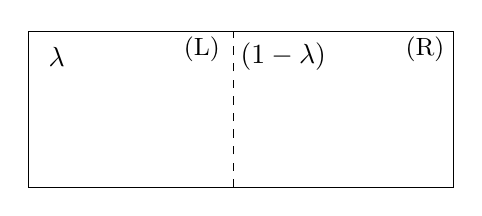
\begin{tikzpicture}[scale=0.9]
  \draw (0,0) rectangle (6,2.2);
  \draw[dashed] (2.9,0) -- (2.9,2.2);
  \node at (0.4,1.85) {$\lambda$};
  \node at (2.45,1.95) {\small (L)};
  \node at (3.6,1.85) {$(1-\lambda)$};
  \node at (5.6,1.95) {\small (R)};
\end{tikzpicture}
\end{minipage}
\begin{minipage}{0.48\textwidth}
-- jeden systém, myšleně rozdělím na 2, nechť je interakce na spol.\ povrchu zanedbatelná
\end{minipage}
\[
  (*)\quad S = S(U,V,N) = S(\lambda U,\lambda V,\lambda N) + S\big[(1-\lambda)U,(1-\lambda)V,(1-\lambda)N\big]
\]
$\Rightarrow$ nelze splnit jinak než pro homog.\ funkci(?)
\[ S(U,V,N) = \lambda S(U,V,N) + (1-\lambda)S(U,V,N) \quad\checkmark \]
\begin{itemize}[nosep]
  \item pokud povrchové jevy hrají roli, bude platit
  \[ S_{\text{celk}}(U,V,N) = S_L(\lambda U,\dots) + S_R((1-\lambda)U,\dots) \]
  kde $S_{\text{celk}}$, $S_L$ \& $S_R$ jsou jiné funkce $\Rightarrow$ \pozor{aditivita homogenitu/extenzivitu nevyžaduje!}
\end{itemize}
\end{priklad}
\noindent\rule{\linewidth}{0.4pt}

\begin{veta}[Postulát 5]
\textcolor{NavyBlue}{Změna entropie mezi rovnovážnými stavy spojená s izotermickým procesem je v limitě $T\to 0$ nulová.}
\end{veta}
\begin{minipage}{0.55\textwidth}\small
Motivace: $G = \dots + T s_0$, v neizotermickém procesu tedy změna $G$ závisí na neurčené konstantě $s_0$; Nernst říká $S(T\to 0)$ je konst.\ nezávislá na ost.\ TD proměnných\dots\ Mohu tedy volit $S(T=0) = 0$?
\end{minipage}
\begin{minipage}{0.43\textwidth}\color{NavyBlue}
$\Big(\pdv{U}{S}\Big)_{X_i} = 0$ \ \textcolor{black}{\pozor{!} má smysl pouze pro kvant.\ systémy, viz $S_{\text{id}} = \log T$ \pozor{!}} \\
\quad$\Updownarrow$ \quad $S(T) = \displaystyle\int_0^T\frac{\dbar Q}{T'}$
\end{minipage}

\medskip
Alt:
\begin{enumerate}[label=\arabic*)]
  \item $\displaystyle\lim_{T\to 0^+}S(T) = 0$
  \item $\displaystyle\lim_{T\to 0^+}\Big(\pdv{S}{X}\Big)_T = 0$ \quad \dots\ izoterma $T = 0$ splývá s adiabatou $\Leftrightarrow$ u abs.\ nuly je $S$ pouze fcí teploty \\
  \quad $\to$ také neplatí vždy
  \item $T = 0$ je nedosažitelná konečným počtem kroků \dots\ jako jediné tvrzení zřejmě velmi univerzálně platí, ale s původním Nernstovým postulátem má málo společného
\end{enumerate}
%----------------------------------------------------------------------
\strana{L04a-5}
\underline{Pozn 3:} V rovnovážném stavu si systém nepamatuje svoji historii $\leftrightarrow$ v axiomatické formulaci je toto zajištěno tím, že \underline{diferenciály $\forall$ stavových funkcí jsou úplné} $\Rightarrow$ jejich změna mezi rovnovážnými stavy je popsána způsobem, který je na této změně nezávislý
\[ \Downarrow \]

\subsection*{Clausiova/Kelvinova $\xrightarrow{\ S(U,X)\ }$ Gibbsova termodynamika}
\begin{itemize}
  \item Kelvin, Clausius -- systém je popisován skrze interakci s okolím
  \item Gibbs -- systém je studován skrze jeho rovnovážné stavy; $S = S(U,V,N_i,\{\xi_i\})$ nijak neodkazuje na okolí \textcolor{NavyBlue}{(okolí vstupuje do hry \uv{nastavením} vnějších vazeb -- celk.\ energie, počet částic, objem, \dots)}
  \begin{itemize}
    \item[--] $S(U,V,N)$ je (rovnovážná) stavová funkce, nezávisí na tom, jak se systém do daného stavu dostal, interakce s okolím je zapomenuta,
    \[
      \vzorec{\dd U = T\dd S + \sum y_i\dd X_i} \qquad \vzorec{\dd S = \frac1T\dd U - \sum\frac{y_i}{T}\dd X_i}
    \]
    jsou obecně platné tvary diferenciálů bez ohledu na vratnost procesu
    \item[--] otázkou je nyní spíše definice tepla a práce, ale k tomu se ještě vrátíme
  \end{itemize}
\end{itemize}

